\subsection{Desempeño en el conjunto de prueba}

El hardware registrado para las corridas fue Tesla T4. Los frameworks y sus versiones se registraron por ejecución junto con la plataforma y la versión de Python.

Se completaron diez entrenamientos y se evaluaron sus checkpoints seleccionados sobre las mismas 2.633 imágenes de prueba. Cada evaluación produjo probabilidades, etiquetas, métricas por clase y una matriz de confusión. La Tabla~\ref{tab:results} presenta la media y desviación estándar muestral de las cinco semillas. Los valores individuales se conservan en el consolidado y en los CSV por corrida.

\begin{table}[t]\caption{Resultados de prueba sobre cinco semillas.}\label{tab:results}\centering\begin{tabular}{lll}\toprule Métrica & CNN & YOLO26n-cls\\\midrule

F1 macro & 0{,}7077 $\pm$ 0{,}0234 & 0{,}7478 $\pm$ 0{,}0537\\

Exactitud & 0{,}7322 $\pm$ 0{,}0266 & 0{,}7676 $\pm$ 0{,}0538\\

Precisión macro & 0{,}7279 $\pm$ 0{,}0166 & 0{,}7685 $\pm$ 0{,}0496\\

Recall macro & 0{,}7160 $\pm$ 0{,}0212 & 0{,}7534 $\pm$ 0{,}0509\\

\bottomrule\end{tabular}\end{table}

YOLO26n-cls obtuvo el mayor F1 macro medio bajo este protocolo. La diferencia media YOLO menos CNN fue 0{,}0400. El valor p bilateral fue 0{,}1875. Con cinco diferencias pareadas, la resolución mínima de la prueba es 0{,}0625, por lo que este diseño carece de resolución para alcanzar el umbral convencional de 0{,}05 mediante esta prueba exacta.

\begin{figure}[t]\centering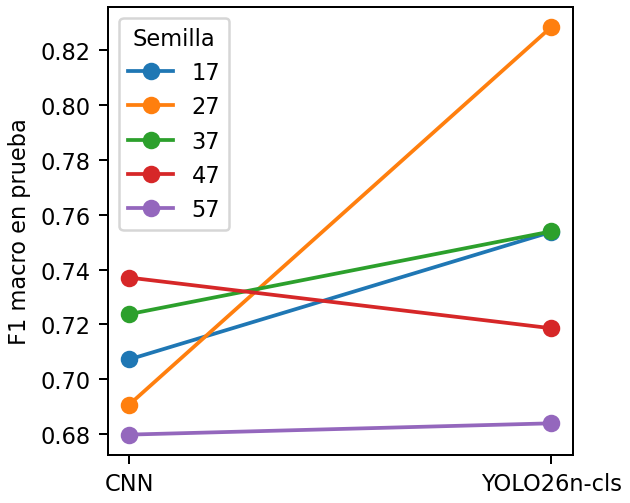
\includegraphics[width=\columnwidth]{paired_f1.png}\caption{F1 macro de prueba por semilla. Cada segmento conecta las corridas de la misma semilla.}\label{fig:paired}\end{figure}

La Fig.~\ref{fig:paired} permite examinar si la diferencia entre arquitecturas es consistente entre semillas y cómo se compara con la dispersión de cada modelo. Cada pareja usa la misma semilla y la misma secuencia de aumentos durante las épocas compartidas. Las arquitecturas consumen secuencias distintas al inicializar sus parámetros. La variabilidad entre semillas se refiere al entrenamiento y conserva fija la muestra de prueba.

\subsection{Comportamiento de aprendizaje}

\begin{figure*}[t]\centering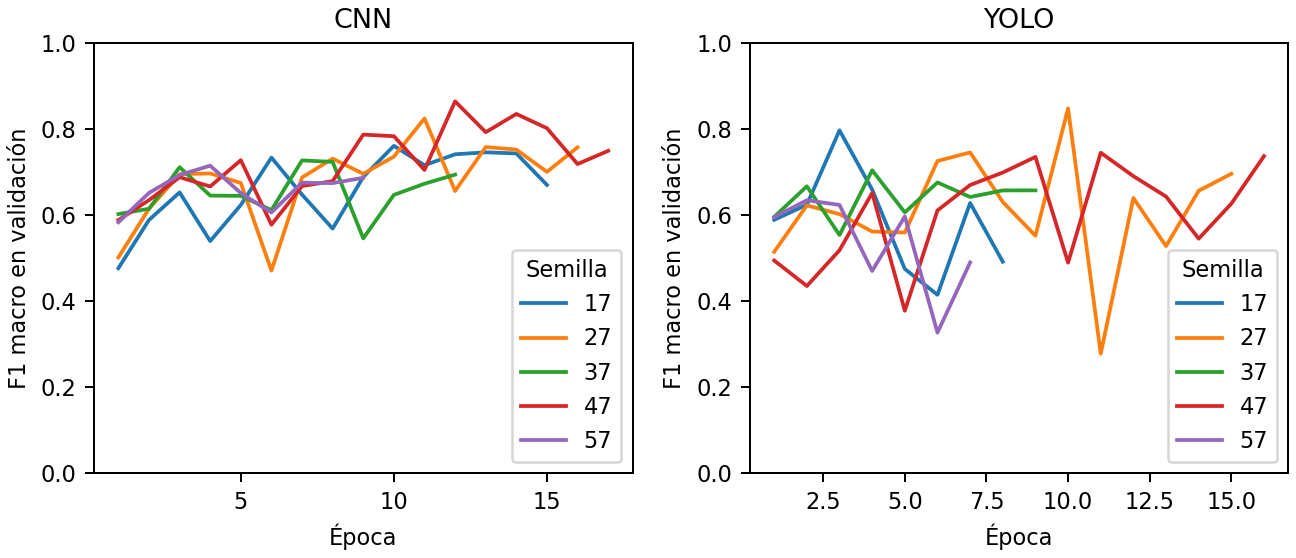
\includegraphics[width=\textwidth]{learning_curves.png}\caption{F1 macro de validación durante los cinco entrenamientos por arquitectura.}\label{fig:learning}\end{figure*}

\begin{figure*}[t]\centering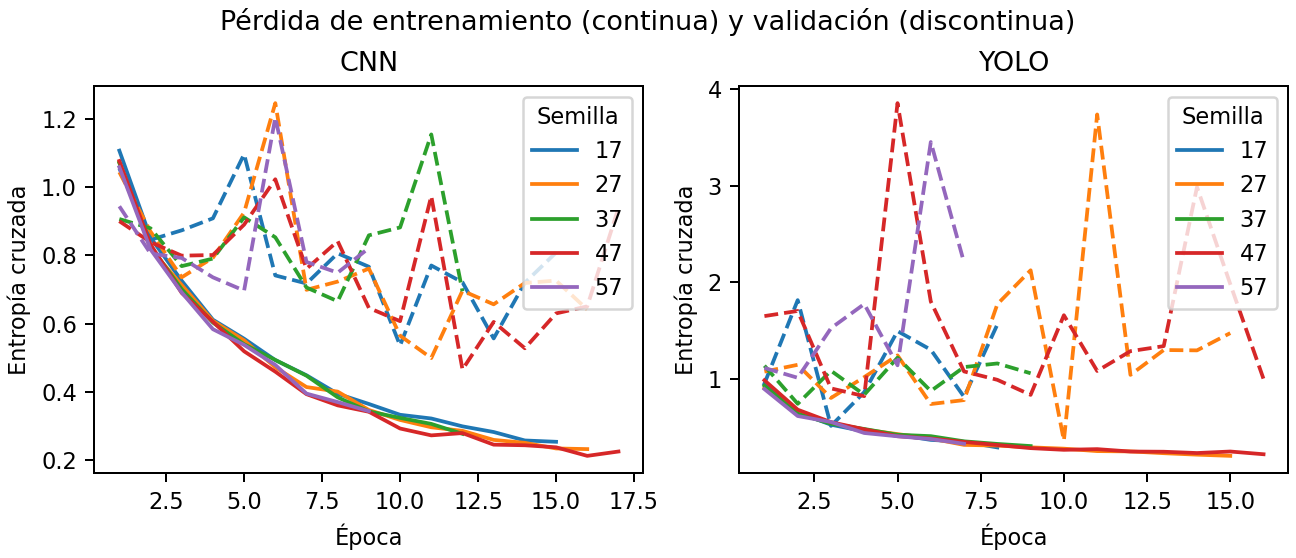
\includegraphics[width=\textwidth]{loss_curves.png}\caption{Pérdidas de entrenamiento y validación por época y semilla.}\label{fig:loss}\end{figure*}

Las Figs.~\ref{fig:learning} y~\ref{fig:loss} muestran la evolución de las corridas hasta la parada. Se comparan las curvas de validación con la reducción de pérdida de entrenamiento para identificar oscilaciones y posibles diferencias de generalización. El criterio común seleccionó el checkpoint por F1 macro de validación. Una reducción adicional de la pérdida de entrenamiento después del máximo de F1 puede coexistir con una degradación de la validación.

En CNN, el F1 macro medio de validación de los checkpoints seleccionados fue 0{,}7776 y el de la última época fue 0{,}7109. Esta comparación describe la evolución de validación y respalda conservar el checkpoint seleccionado antes de evaluar prueba.

En CNN, las épocas finales de las cinco semillas fueron 15, 16, 12, 17, 9. Los checkpoints seleccionados correspondieron a las épocas 10, 11, 7, 12, 4, respectivamente. La elección conserva el presupuesto máximo compartido y permite que la parada temprana determine duraciones distintas según la trayectoria de validación.

En YOLO26n-cls, el F1 macro medio de validación de los checkpoints seleccionados fue 0{,}7450 y el de la última época fue 0{,}6139. Esta comparación describe la evolución de validación y respalda conservar el checkpoint seleccionado antes de evaluar prueba.

En YOLO26n-cls, las épocas finales de las cinco semillas fueron 8, 15, 9, 16, 7. Los checkpoints seleccionados correspondieron a las épocas 3, 10, 4, 11, 2, respectivamente. La elección conserva el presupuesto máximo compartido y permite que la parada temprana determine duraciones distintas según la trayectoria de validación.

\subsection{Eficiencia computacional}

\begin{table}[t]\caption{Costo computacional de las cinco corridas.}\label{tab:time}\centering\begin{tabular}{lll}\toprule Medida & CNN & YOLO26n-cls\\\midrule

Entrenamiento (s) & 359{,}4227 $\pm$ 84{,}8609 & 350{,}1515 $\pm$ 131{,}8539\\

Latencia p50 (ms) & 1{,}5233 $\pm$ 0{,}2536 & 6{,}3146 $\pm$ 0{,}1105\\

Latencia p95 (ms) & 2{,}2994 $\pm$ 0{,}6333 & 8{,}0960 $\pm$ 1{,}1326\\

\bottomrule\end{tabular}\end{table}

La Tabla~\ref{tab:time} muestra el costo observado. CNN presentó la menor latencia mediana media bajo el protocolo de lote uno. Estos tiempos incluyen los pasos de inferencia definidos en métodos y dependen del hardware, el framework y las condiciones de carga. El tiempo total de entrenamiento también depende de cuántas épocas completó cada corrida. Se conservaron ambas medidas para diferenciar costo por predicción y costo de aprendizaje.

\begin{figure}[t]\centering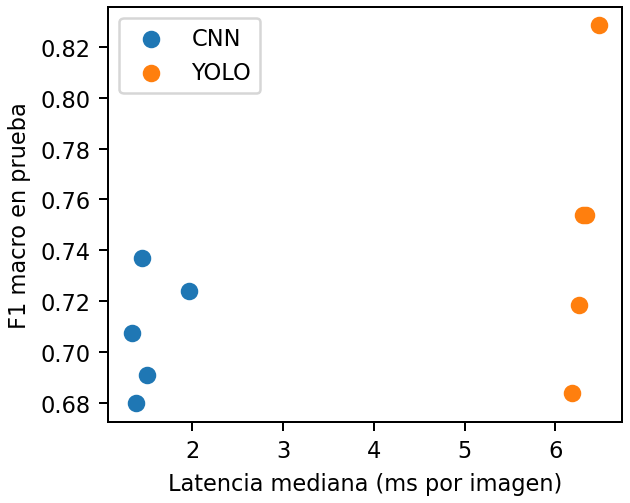
\includegraphics[width=\columnwidth]{f1_latency.png}\caption{F1 macro frente a latencia mediana de inferencia. Cada punto corresponde a una semilla.}\label{fig:latency}\end{figure}

La Fig.~\ref{fig:latency} combina las métricas predictiva y computacional para examinar compromisos entre exactitud y tiempo. La nube de puntos informa sobre la dispersión observada bajo la misma partición. La comparación no incluye compilación a ONNX o TensorRT, y cualquier extensión a otros equipos requiere repetir la medición con el mismo protocolo.

\subsection{Errores por clase y mapas de activación}

\begin{table}[t]\caption{Métricas medias por clase en prueba.}\label{tab:class}\centering\begin{tabular}{llrrr}\toprule Modelo & Clase & P & R & F1\\\midrule

CNN & cyst & 0{,}7310 & 0{,}9034 & 0{,}8077\\

CNN & normal & 0{,}7310 & 0{,}7393 & 0{,}7235\\

CNN & stone & 0{,}5955 & 0{,}4389 & 0{,}4858\\

CNN & tumor & 0{,}8540 & 0{,}7826 & 0{,}8140\\

YOLO26n-cls & cyst & 0{,}7375 & 0{,}9666 & 0{,}8347\\

YOLO26n-cls & normal & 0{,}7660 & 0{,}7306 & 0{,}7436\\

YOLO26n-cls & stone & 0{,}7074 & 0{,}5028 & 0{,}5843\\

YOLO26n-cls & tumor & 0{,}8630 & 0{,}8136 & 0{,}8284\\

\bottomrule\end{tabular}\end{table}

La Tabla~\ref{tab:class} permite evaluar el aporte de cada clase al promedio macro. Sus precisiones y recalls se interpretan junto con las matrices de confusión para distinguir falsos positivos y falsos negativos. Las diferencias entre clases pueden reflejar apariencia, tamaño de muestra, mezcla de modalidades o calidad de las etiquetas. El experimento carece de metadatos suficientes para atribuirlas a una sola causa.

\begin{figure}[t]\centering\includegraphics[width=\columnwidth]{cnn-17/confusion.png}\caption{Matriz de confusión de CNN, semilla 17. Filas con etiqueta real y columnas con predicción.}\label{fig:conf-cnn}\end{figure}

En la corrida ilustrativa de CNN con semilla 17, la confusión dirigida más frecuente fue stone como normal, con 169 imágenes. La Fig.~\ref{fig:conf-cnn} muestra todos los conteos. Esta semilla se fijó para las figuras ilustrativas antes de consultar la prueba y el resumen principal incluye las cinco corridas.

\begin{figure}[t]\centering\includegraphics[width=\columnwidth]{yolo-17/confusion.png}\caption{Matriz de confusión de YOLO26n-cls, semilla 17. Filas con etiqueta real y columnas con predicción.}\label{fig:conf-yolo}\end{figure}

En la corrida ilustrativa de YOLO26n-cls con semilla 17, la confusión dirigida más frecuente fue stone como cyst, con 151 imágenes. La Fig.~\ref{fig:conf-yolo} muestra todos los conteos. Esta semilla se fijó para las figuras ilustrativas antes de consultar la prueba y el resumen principal incluye las cinco corridas.

\begin{figure}[t]\centering\includegraphics[width=\columnwidth]{cnn-17/gradcam.png}\caption{Grad-CAM de la CNN, semilla 17, en la tercera convolución. El mapa se calcula respecto a la clase predicha.}\label{fig:gradcam}\end{figure}

El mapa Grad-CAM \cite{gradcam} de la Fig.~\ref{fig:gradcam} usa el gradiente de la clase predicha sobre la tercera convolución. Esta capa conserva una cuadrícula espacial de 7 por 7, mientras que la cuarta alcanza una resolución muy reducida. El mapa ofrece una localización gruesa de las activaciones relacionadas con la salida. La selección de la imagen sigue la regla de error de mayor confianza de la semilla 17, o la primera imagen si esa corrida carece de errores. El mapa requiere lectura junto con la imagen, su etiqueta y su predicción.


En promedio, Stone obtuvo el menor F1 de las cuatro clases: 0{,}4858 en la CNN y 0{,}5843 en YOLO26n-cls. Su recall medio fue 0{,}4389 y 0{,}5028, respectivamente. Este resultado identifica una dificultad persistente que el promedio global puede ocultar. Las cifras corresponden a las etiquetas del conjunto y deben interpretarse junto con su procedencia heterogénea.

El ejemplo de la Fig.~\ref{fig:gradcam}, \texttt{kidney-stone-0066.jpg}, está etiquetado como Stone y fue clasificado como Cyst con puntuación softmax de 0{,}9998. El mapa resalta bandas curvas periféricas del tercio inferior. Esta distribución permite plantear una revisión de posibles atajos visuales asociados al encuadre. El mapa, por sí solo, no demuestra la causa del error ni valida una localización anatómica. Las salidas softmax de este estudio no fueron calibradas.
